\documentclass[
11pt, % The default document font size, options: 10pt, 11pt, 12pt
%codirector, % Uncomment to add a codirector to the title page
]{charter} 

% El títulos de la memoria, se usa en la carátula y se puede usar el cualquier lugar del documento con el comando \ttitle
\titulo{Cadenas de procesamiento re-configurables en SoC/MPSoC } 

% Nombre del posgrado, se usa en la carátula y se puede usar el cualquier lugar del documento con el comando \degreename
\posgrado{Especialización en Sistemas Embebidos} 
%\posgrado{Carrera de Especialización en Internet de las Cosas} 
%\posgrado{Carrera de Especialización en Intelegencia Artificial}
%\posgrado{Maestría en Sistemas Embebidos} 
%\posgrado{Maestría en Internet de las cosas}

% Tu nombre, se puede usar el cualquier lugar del documento con el comando \authorname
\tituloAutor{Ing. }
\autor{Carlos Jorge Maffrand} 

% El nombre del director y co-director, se puede usar el cualquier lugar del documento con el comando \supname y \cosupname y \pertesupname y \pertecosupname
\tituloDirector{Esp. Ing. }
\director{Gonzalo Lavigna}
\pertenenciaDirector{FIUBA}

% Nombre del cliente, quien va a aprobar los resultados del proyecto, se puede usar con el comando \clientename y \empclientename
\tituloCliente{Mg. Ing. }
\cliente{Franco Alcaraz}
\empresaCliente{INVAP}

% Nombre y pertenencia de los jurados, se pueden usar el cualquier lugar del documento con el comando \jurunoname, \jurdosname y \jurtresname y \perteunoname, \pertedosname y \pertetresname.
\juradoUno{Nombre y Apellido (1)}
\pertenenciaJurUno{pertenencia (1)} 
\juradoDos{Nombre y Apellido (2)}
\pertenenciaJurDos{pertenencia (2)}
\juradoTres{Nombre y Apellido (3)}
\pertenenciaJurTres{pertenencia (3)}
 
\fechaINICIO{24 de junio de 2021}		%Fecha de inicio de la cursada de GdP \fechaInicioName
\fechaFINALPlan{24 de agosto de 2021} 	%Fecha de final de cursada de GdP
\fechaFINALTrabajo{24 de junio de 2022}	%Fecha de defensa pública del trabajo final

% Definición de constantes que van a ser utilizadas dentro del proyectos
\costoProyecto{4.429.000} 
\esfuerzoProyecto{800}

\begin{document}

\maketitle
\thispagestyle{empty}
\pagebreak

\thispagestyle{empty}
{\setlength{\parskip}{0pt}
\tableofcontents{}
}
\pagebreak

\section*{Registros de cambios}
\label{sec:registro}

\begin{table}[ht]
\label{tab:registro}
\centering
\begin{tabularx}{\linewidth}{@{}|c|X|c|@{}}
\hline
\rowcolor[HTML]{\tablecolor} 
Revisión & \multicolumn{1}{c|}{\cellcolor[HTML]{\tablecolor}Detalles de los cambios realizados} & Fecha      \\ \hline
0      & Creación del documento                                 &\fechaInicioName \\ \hline
1      & Se genera la primera versión de los incisos 1, 2, 3, 4 y 5.                 & 04 de julio de 2021 \\ \hline
2      & Se genera la primera versión de los incisos 6, 7, 8 y 9. & 08 de julio de 2021 \\ \hline
3      & Se genera la primera versión de los incisos 10, 11 y 12. & 17 de julio de 2021 \\ \hline
4      & Se genera la primera versión de los incisos 13, 14 y 15. & 31 de julio de 2021 \\ \hline
\end{tabularx}
\end{table}

\pagebreak

\section*{Acta de constitución del proyecto}
\label{sec:acta}

\begin{flushright}
Buenos Aires, \fechaInicioName
\end{flushright}

\vspace{2cm}

Por medio de la presente se acuerda con el Ing. \authorname\hspace{1px} que su Trabajo Final de la \degreename\hspace{1px} se titulará ``\ttitle'', consistirá en \textcolor{black}{implementar un sistema que permita seleccionar bloques de procesamiento almacenado en memoria, realizar re-configuración dinámica en lógica programable y ofrecer un entorno de pruebas para el filtro seleccionado. Este entorno de pruebas debe ser capaz de generar una onda de excitación para el filtro, adquirir los datos filtrados y generar reportes de pruebas. Este desarrollo tiene como finalidad evaluar el uso de bancos de filtros mediante re-configuración dinámica de lógica programable para aplicaciones satelitales y de radar}, y tendrá un presupuesto preliminar estimado de \textcolor{black}{\projecteffort} horas de trabajo y \textcolor{black}{\$ \projectcost}, con fecha de inicio \fechaInicioName\hspace{1px} y fecha de presentación pública \fechaFinalName.

Se adjunta a esta acta la planificación inicial.

\vfill

% Esta parte se construye sola con la información que hayan cargado en el preámbulo del documento y no debe modificarla
\begin{table}[ht]
\centering
\begin{tabular}{ccc}
\begin{tabular}[c]{@{}c@{}}Dr. Ing. Ariel Lutenberg \\ Director posgrado FIUBA\end{tabular} & \hspace{2cm} & \begin{tabular}[c]{@{}c@{}}\clienttittle \clientename \\ \empclientename \end{tabular} \vspace{2.5cm} \\ 
\multicolumn{3}{c}{\begin{tabular}[c]{@{}c@{}} \directortittle \supname \\ Director del Trabajo Final\end{tabular}} \vspace{2.5cm} \\
%\begin{tabular}[c]{@{}c@{}}\jurunoname \\ Jurado del Trabajo Final\end{tabular}     &  & \begin{tabular}[c]{@{}c@{}}\jurdosname\\ Jurado del Trabajo Final\end{tabular}  \vspace{2.5cm}  \\
%\multicolumn{3}{c}{\begin{tabular}[c]{@{}c@{}} \jurtresname\\ Jurado del Trabajo Final\end{tabular}} \vspace{.5cm}                                                                     
\end{tabular}
\end{table}

\clearpage

\section{1. Descripción técnica-conceptual del proyecto a realizar}
\label{sec:descripcion}

En los desarrollos tecnológicos, tanto aeroespaciales como de radares, es muy frecuente la utilización de procesamiento digital de señales en dispositivos de lógica programable. En consecuencia, dado los elevados costos de los lanzamientos, misiones espaciales y desarrollos de defensa, es necesaria la utilización eficiente de los recursos. Por lo que, mediante la re-configuración parcial, se podría reducir el número de dispositivos de lógica programable utilizados en futuros desarrollos.

El sistema propuesto en este plan de trabajo permitirá hacer una evaluación del uso de técnicas de re-configuración dinámica parcial en dispositivos de lógica programable para aplicaciones espaciales y de defensa.

Las \ttitle permiten seleccionar filtros de procesamiento, previamente generados, de un banco de filtros almacenado en memoria, realizar la re-configuración dinámica y evaluar el funcionamiento del banco seleccionado. Como componente principal, el dispositivo a desarrollar cuenta con un System on Chip (SoC) o Multi Processor System on Chip (MPSoC).

En la Figura \ref{fig:diagBloques} se muestra un diagrama de bloques en el que se observan las funcionalidades principales de la aplicación a desarrollar. De la misma, se desprende que el objetivo de la aplicación es generar un entorno de software-HDL que permita la selección de bancos de filtros que re-configuran la lógica programable del SoC/MPSoC.

\begin{figure}[h]
\raggedleft
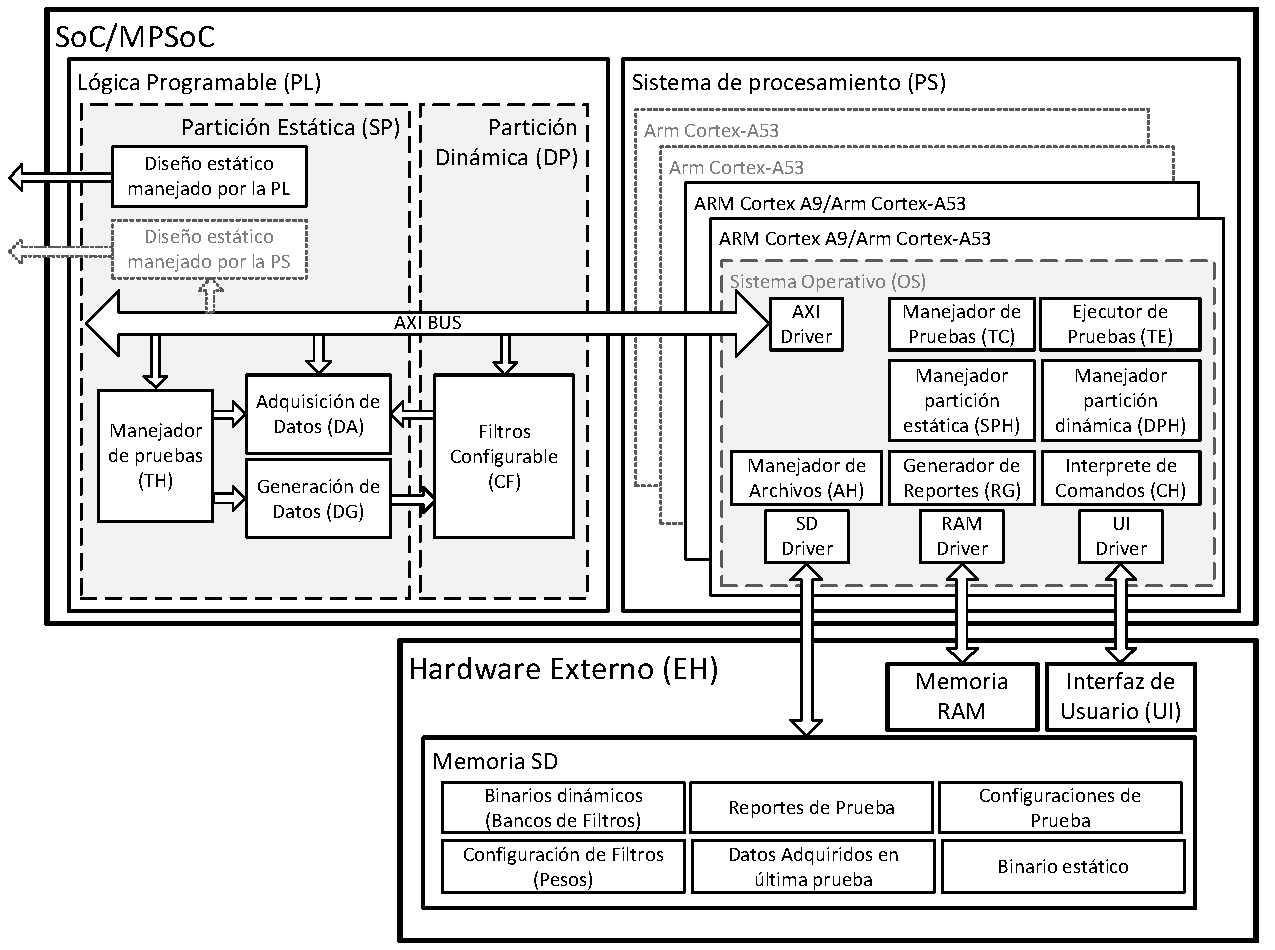
\includegraphics[width=1.05\textwidth]{./Figuras/DiagamaCPR_grande.pdf}
\caption{Diagrama en bloques.}
\label{fig:diagBloques}
\end{figure}

El entorno de pruebas se debe implementar haciendo uso de un kit de desarrollo que contenga un SoC o MPSoC de serie 7 o superior de la marca Xilinx. Por lo que, se deben establecer los mecanismos de re-configuración mediante el entorno de desarrollo Vivado.

El dispositivo debe constar de los principales bloques constitutivos:
\begin{itemize}
	\item Interfaz de usuario (UI): debe proveer al operador un modo de configurar el filtro de procesamiento empleado en el dispositivo, disparar la ejecución de pruebas y obtener los archivos de reporte. Adicionalmente, el operador debe poder actualizar los archivos que conforman el banco de filtros con los que se puede configurar la lógica programable (PL).
	\item Sistema de procesamiento (PS): debe contar con un sistema operativo que permita la ejecución de diferentes aplicaciones. Las mismas tienen como funcionalidades principales: controlar los periféricos del procesador, realizar la re-configuración de la PL, generar y administrar los reportes de pruebas, administrar el banco de filtros, configurar las pruebas a realizar y gestionar la comunicación con la PL mediante el bus AXI.
	\item Lógica programable (PL): en la misma se debe disponer de una parte estática donde se instancia una lógica de generación de estímulos y adquisición de datos para la realización de las pruebas sobre los filtros. Por otro lado, en la PL debe existir una sección configurable donde se deben instanciar los bloques de procesamiento.
	\item Memoria estática (SD): espacio de memoria donde se se deben almacenar el banco de filtros, los reportes de las pruebas ejecutadas, archivos de configuración del sistema y los datos de las pruebas recientemente realizadas por el usuario.
	\item Memoria RAM: a ser utilizada para la generación de reportes.
\end{itemize}
 
\clearpage

\section{2. Identificación y análisis de los interesados}
\label{sec:interesados}

\begin{table}[ht]
\begin{center}
\begin{tabularx}{\linewidth}{@{}|l|X|X|l|@{}}
\hline
\rowcolor[HTML]{\tablecolor} 
Rol           & Nombre y Apellido & Organización 	& Puesto 	\\ \hline
%Auspiciante   &  - 				  & -              	& -        	\\ \hline
Cliente       & \clientename      &\empclientename	& -       	\\ \hline
%Impulsor      & - &\empclientename 	& -       	\\ \hline
Responsable   & \authorname       & FIUBA        	& Alumno 	\\ \hline
%Colaboradores & -                 & -             	& -       	\\ \hline
Orientador    & \supname	      & \pertesupname 	& Director Trabajo Final \\ \hline
%Equipo        & -			      & -            	& -       	\\ \hline
%Opositores    & -                 & -            	& -      	\\ \hline
Usuario final & Ingeniero de desarrollo                & \empclientename	& -       	\\ \hline
\end{tabularx}
\caption{Identificación de los interesados.}
\label{tab:interesados}
\end{center}
\end{table}

\begin{itemize}
	\item Cliente: \clientename, es un profesional altamente calificado en la industria aeroespacial y defensa.
	\item Orientador: \supname, es egresado de la Especialización en Sistemas Embebidos de la FIUBA, posee muchos años de experiencia desarrollando proyectos en la industria aeroespacial y de defensa. Probablemente esté viviendo en Europa, por lo que hay que tener en cuenta ese hecho cuando se decida contactarlo.
	%\item Usuario final: profesional que aún no está definido por \empclientename.
\end{itemize}

\section{3. Propósito del proyecto}
\label{sec:proposito}

El propósito de este proyecto es realizar una evaluación tecnológica de la re-configuración dinámica de dispositivos de lógica programable, con el fin de establecer criterios de uso para desarrollos aeroespaciales y de radares. Adicionalmente, el cliente desea adquirir la capacidad de desarrollar una aplicación con esa tecnología de modo de subir el Technology Readiness Level (TRL) que se posee dentro de \empclientename.

\section{4. Alcance del proyecto}
\label{sec:alcance}

El proyecto descripto en este plan de trabajo deberá brindar las siguientes funcionalidades:

\begin{itemize}
	\item Administrar un banco de filtros previamente generados en un sistema de archivos.
	\item Seleccionar el filtro que se planea utilizar.
	\item Realizar la re-configuración parcial de la lógica programable del SoC/MPSoC, implementando el filtro previamente seleccionado.
	\item Configurar el entorno de pruebas presente en la parte estática de la PL.
	\item Ejecutar pruebas configuradas en las cadenas de filtros elegidas.
	\item Adquirir los datos generados en las pruebas.
	\item Emitir reportes sobre las pruebas ejecutadas.
\end{itemize}

El presente proyecto no incluye las siguientes funcionalidades:
\begin{itemize}
	\item Generar archivos binarios de filtros para la configuración dinámica de la PL.
	\item Rutinas de verificación, validación y evaluación de performance de las pruebas realizadas en los filtros configurados en la PL.
	\item Evaluación de los tiempos de re-configuración.
	\item Almacenamiento de grandes volúmenes de datos.
\end{itemize}

\section{5. Supuestos del proyecto}
\label{sec:supuestos}

Se supone que el software correrá en una plataforma de hardware tipo System on Chip de la línea Xilinx Zynq (ARM+FPGA).

El responsable del proyecto dispone de una placa ZedBoard para la realización del desarrollo. Con el fin de que el banco de pruebas sea implementado en una tecnología más moderna, se debe evaluar si INVAP dispone de un hardware de desarrollo que contenga un MPSoC.

Se asume que se dispondrá de la plataforma de desarrollo durante el tiempo que dure el proyecto para poder depurar el diseño sobre el hardware.

Se va a hacer uso de Vivado y las herramientas adicionales de dicho entornos de desarrollo para dispositivos de la marca Xilinx. Por lo que, se supone que se cuentan con las licencias para tal fin.

Se supone que se va a hacer uso de HDL Coder para obtener los filtros para el prototipo del sistema. Por lo que, se supone que se cuentan con las licencias para su uso.

\clearpage

\section{6. Requerimientos}
\label{sec:requerimientos}

Para comprender los requerimientos del proyecto se enumeran los siguientes acrónimos:

\begin{itemize}
		\item API: Application Programming Interface.
		\item AXI: Advanced eXtensible Interface.
		\item HDL: Hardware Description Language.
		\item MPSoC: Multi-Processor System on a Chip.
		\item PL: Programmable Logic en un SoC u MPSoC.
		\item PS: Processing System en un SoC o MPSoC.
		\item SoC: System on a Chip.
		\item TBD: To Be Defined.
		\item UART: Universal Asynchronous Receiver-Trasmitter.
		\item VHDL: Very High Speed Integrated Circuit Hardware Description Language.
\end{itemize}

\begin{enumerate}	
	\item Requerimientos de interfaces externas
		\begin{enumerate}
			\item El sistema debe implementar una interfaz de usuario por consola.
			\item La consola de interfaz de usuario debe ser implementada mediante UART y/o Ethernet.
			\item En la partición estática de la PL se debe implementar una interfaz serie que tenga funcionamiento independiente de la PS.
			\item En la partición estática de la PL se debe implementar una interfaz serie que tenga funcionamiento controlado por la PS.
		\end{enumerate}
	
	\item Requerimientos de interfaces internas	
		\begin{enumerate}
			\item El software alocado en la PS debe comunicarse con la PL mediante una interfaz AXI.
			\item El software alocado en la PS debe implementar un sistema de archivos en una memoria SD.
			\item El software alocado en la PS debe manejar una interfaz con una memoria RAM.
			\item El software alocado en la debe tener una interfaz para re-configurar dinámicamente la porción de la PL dedicada para tal fin.
			\item El software alocado en la PS debe tener una interfaz para configurar el sector de PL estático.
		\end{enumerate}
	
	\item Requerimientos de almacenamiento de información (sistema de archivos)
	\begin{enumerate}
		\item El sistema debe almacenar reportes de las pruebas ejecutadas en el sistema de archivos.
		\item El sistema debe almacenar pre-configuraciones para el entorno de pruebas en el sistema de archivos.
		\item El sistema debe almacenar el archivo de configuración del sector estático de la PL  en el sistema de archivos.
		\item El sistema debe almacenar al menos dos archivos binarios (filtros previamente generados) de configuración del sector dinámico de la PL  en el sistema de archivos.
		\item El sistema debe almacenar archivos de configuración (pesos de los filtros) del sector dinámico de la PL  en el sistema de archivos.
		\item El sistema debe almacenar los datos obtenidos de al menos la última ejecución de pruebas en el sistema de archivos.
	\end{enumerate}
	
	\item Requerimientos generales de HDL
	\begin{enumerate}
		\item La lógica programable debe ser codificada en lenguaje VHDL.
		\item En la PL se debe generar una partición para uso dinámico.
		\item En la PL se debe generar una partición para uso estático.
		\item Para la comunicación entre bloques de lógica se debe utilizar el bus AXI.
	\end{enumerate}
	
	\item Requerimientos de HDL estático
	\begin{enumerate}		
		\item En la partición estática se debe implementar una funcionalidad de lógica programable que sea independiente de la PS.
		\item En la partición estática se debe implementar una funcionalidad de lógica programable que sea manejada por la PS.
		\item En la partición estática se debe implementar una funcionalidad de lógica programable para la generación de señales de excitación de los filtros.
		\item En la partición estática se debe implementar una funcionalidad de lógica programable para la adquisición de datos generados por las salidas de los filtros.
		\item En la partición estática se debe implementar una funcionalidad de lógica programable que permita la configuración de las pruebas a realizar en el banco de filtros.
	\end{enumerate}
	
	\item Requerimientos de configuración del entorno de pruebas
	\begin{enumerate}
		\item El sistema debe instanciar el archivo de configuración de sector estático de la PS.
		\item El sistema debe permitir al usuario la selección del archivo de configuración de sector dinámico de la PL.
		\item El sistema debe permitir al usuario la solicitud de re-configuración dinámica de la porción de la PL dedicada a tal fin.
		\item El sistema debe ejecutar la re-configuración dinámica.
		\item El sistema debe permitir al usuario la configuración de la prueba en la parte estática de la PS haciendo uso de los siguientes parámetros:
		\begin{enumerate}[a.]
			\item Duración de la prueba.
			\item Ancho de palabra del filtro configurado.
			\item Tipo de onda generada para la prueba.
		\end{enumerate}
		\item El sistema debe escribir los registros de configuración de los bloques implementados en la parte estática de la PS:
		 \begin{enumerate}[a.]
			\item Generación de datos de excitación.
			\item Configuración de test.
			\item Adquisición de datos.
		\end{enumerate}
		\item El sistema debe permitir al usuario la opción de ejecutar pruebas sin generar reportes o almacenar los datos generados. 
		\item El sistema debe permitir al operador actualizar los archivos que conforman el banco de filtros. Dichos archivos son binarios previamente generados en la herramienta de síntesis de HDL.	
	\end{enumerate}
		
	\item Requerimientos funcionales (ejecución de pruebas)
	\begin{enumerate}
		\item El sistema debe permitir al usuario la solicitud de ejecución de pruebas en la PL. Tales pruebas pueden ser:
		\begin{enumerate}[a.]
			\item Respuesta de filtro a estímulos generados.
			\item Comportamiento de la lógica en la PL estática cuando se realiza la configuración dinámica.
			\item Evaluación del tiempo de re-configuración.
		\end{enumerate}
		\item El software del PS debe escribir los registros de los bloques de lógica programable de generación de datos de excitación, configuración de test y adquisición de datos implementados en la parte estática de la PS de modo tal que se dispare la ejecución de la prueba configurada.
		\item El software del PS debe capturar los datos adquiridos tras la ejecución de la prueba y almacenarlos en el sistema de archivos.
		\item El software del PS debe leer los registros de los bloques de generación de datos de excitación, configuración de test y adquisición de datos.
		\item El software del PS debe generar un reporte de pruebas conteniendo mínimamente la siguiente información:
		\begin{enumerate}[a.]
			\item Fecha de ejecución.
			\item Tiempo de ejecución.
			\item Configuración del sistema de pruebas.
			\item Resultado de las pruebas realizadas.
			\item Filtro seleccionado e instanciado en la PL dinámica.
			\item Versión del archivo instanciado en la PL estática.	
		\end{enumerate}
		\item El software del PS debe controlar que la prueba configurada por el usuario no genere datos superiores a un tamaño de 10 kBytes.
	\end{enumerate}

	\item Requerimientos de rendimiento
	\begin{enumerate}
		\item Una vez iniciada una prueba el reporte de la misma deberá ser generado en menos de un minuto.
	\end{enumerate}

	\item Requerimientos de diseño
	\begin{enumerate}
		\item Se debe utilizar la placa de desarrollo ZedBoard para implementar el desarrollo en un SoC. La placa de desarrollo podría ser modificada por una que contenga un MPSoC, de acuerdo a la disponibilidad de la misma en INVAP.
	\end{enumerate}

	\item Requerimientos de confiabilidad 
	\begin{enumerate}
		\item El sistema debe asegurar su correcto funcionamiento en condiciones normales de operación durante al menos una semana de uso continuo (sin ser reiniciado).
	\end{enumerate}

	\item Requerimientos de documentación
	\begin{enumerate}
		\item Se debe generar un manual de usuario para el sistema de pruebas de bancos de filtros re-configurables.
	\end{enumerate}
\end{enumerate}

\clearpage

\section{7. Historias de usuarios (\textit{Product backlog})}
\label{sec:backlog}

A continuación se presentan cuatro historias de usuario para el proyecto. Vale la pena destacar que los \emph{Story points}, que se le atribuyen a cada una de las historias, son calculados como el número de Fibonacci mayor o igual a la suma de la estimación de carga de trabajo, complejidad y conocimiento previo.

\begin{itemize}
	\item Como \emph{ingeniero de desarrollo} quiero \emph{realizar la configuración dinámica en lógica programable} para evaluar su implementación en diseños complejos.
	
	Carga de trabajo: 5 puntos.
	Complejidad: 3 puntos.
	Conocimiento previo: 3 puntos.
	\begin{center}
		$ 5 + 3 + 3 = 11 \rightarrow 13 $
	\end{center}
	 
	\emph{Story points: 13}, la historia de usuario permite evaluar la complejidad de generar diseños de lógica programable con re-configuración parcial, para con esto evaluar riesgos, ventajas y desventajas de su utilización en proyectos de alto costo y alcance.	
	
	\item Como \emph{ingeniero de desarrollo} quiero \emph{realizar la configuración dinámica en lógica programable} para evaluar el tiempo que toma dicho proceso.

	Carga de trabajo: 3 puntos.
	Complejidad: 2 puntos.
	Conocimiento previo: 2 puntos.
	\begin{center}
		$ 3 + 2 + 2 = 7 \rightarrow 8 $
	\end{center}
	
	\emph{Story points: 8}, la historia de usuario permite dimensionar el tiempo de re-configuración que es un dato de importancia para la evaluación de su uso en sistemas de procesamiento que sean demandantes en su tiempo de ejecución.

	\item Como \emph{ingeniero de desarrollo} quiero \emph{realizar la configuración dinámica en lógica programable} para evaluar el funcionamiento del resto del dispositivo de lógica programable durante el proceso de re-configuración. 
			
	Carga de trabajo: 2 puntos.
	Complejidad: 2 puntos.
	Conocimiento previo: 2 puntos.
	\begin{center}
		$ 2 + 2 + 2 = 6 \rightarrow 8 $
	\end{center}
	
	\emph{Story points: 5}, la historia de usuario permite validar que no se afecta el funcionamiento de la lógica adyacente durante el proceso de re-configuración.

	\item Como \emph{ingeniero de desarrollo} quiero \emph{realizar pruebas de desempeño sobre filtros de procesamiento en hardware} para evaluar y caracterizar su funcionamiento.
			
	Carga de trabajo: 2 puntos.
	Complejidad: 2 puntos.
	Conocimiento previo: 1 puntos.
	\begin{center}
		$ 2 + 2 + 1 = 5 \rightarrow 5 $
	\end{center}

	\emph{Story points: 5}, la historia de usuario permite generar una métrica de funcionamiento de los filtros.

\end{itemize}	

\clearpage

\section{8. Entregables principales del proyecto}
\label{sec:entregables}

Los entregables del proyecto son:

\begin{itemize}
	\item Código fuente c en el repositorio con control de versiones \emph{Github}.
	\item Documentación del código c con \emph{Doxygen}.
	\item Código fuente VHDL en el repositorio con control de versiones \emph{Github}.
	\item Documentación del código VHDL con \emph{TerosHDL}.
	\item Manual de usuario del sistema de pruebas.
	\item Ficha de lecciones aprendidas durante el desarrollo.
	\item Código fuente del firmware y software desarrollado para el PS.
	\item Código fuente del HDL generado para la PL estática.
	\item Código fuente de los HDLs generados para la PL dinámica.
	\item Memoria del Trabajo final.
\end{itemize}

\clearpage

\section{9. Desglose del trabajo en tareas}
\label{sec:wbs}

\begin{enumerate}

	\item Planificación
	\begin{enumerate}
		\item Estudio del problema general (30 horas)
		\item Relevamiento y estudio de los requerimientos (20 horas)
		\item Documentación de requerimientos y especificación del trabajo (20 horas)
		\item Planificación del proyecto (20 horas)		
	\end{enumerate}
	
	\item Proceso de adquisición de conocimientos
	\begin{enumerate}
		\item Estudio del SoC/MPSoC (20 horas)
		\item Estudio de técnicas de re-configuración parcial (40 horas)
		\item Implementación de sistemas operativos y sistemas de archivos en SoC/MPSoC (40 horas)
		\item Estudio de periférico UART (10 horas)
		\item Estudio de periférico Ethernet (20 horas)
		\item Estudio de periférico RAM (30 horas)
		\item Estudio de periférico AXI (10 horas)
		\item Estudio de periférico SD (20 horas)
	\end{enumerate}
	
	\item Desarrollo de aplicaciones
	\begin{enumerate}
		\item Desarrollo de comunicación con PL (40 horas)
		\item Desarrollo de consola intérprete de comandos de usuario (20 horas)
		\item Desarrollo de configurador de PL estática (20 horas)
		\item Desarrollo de configurador de PL dinámica (20 horas)
		\item Desarrollo de configurador y ejecutor de pruebas (API) (40 horas)
		\item Desarrollo de generador de reportes (40 horas)
	\end{enumerate}
	
	\item Desarrollos de HDL
	\begin{enumerate}
		\item Desarrollo de partición PL (40 horas)		
		\item Diseño de puerto de comunicación en PL estática de funcionamiento independiente de la PS (10 horas)
		\item Diseño de puerto de comunicación en PL estática de funcionamiento dependiente de la PS (20 horas)
		\item Diseño del bloque de configuración y ejecución de pruebas (HDL) (40 horas)
		\item Implementación de generador de datos de excitación (30 horas)
		\item Implementación de adquisidor de datos (30 horas)
		\item Implementación de bus AXI e integración general (40 horas)
		\item Implementación de filtros de procesamiento de datos para demo de funcionamiento del sistema (40 horas)
	\end{enumerate}
	
	\item Proceso de cierre
	\begin{enumerate}
		\item Escritura de memoria de Trabajo final (40 horas)
		\item Escritura de manual de usuario (30 horas)
		\item Confección de ficha de lecciones aprendidas (10 horas)
		\item Confección de presentación y defensa pública (10 horas)
	\end{enumerate}	
	
\end{enumerate}

Cantidad total de trabajo estimado para el proyecto: ({\projecteffort} horas)

\clearpage

\section{10. Diagrama de Activity On Node}
\label{sec:AoN}

En la Figura \ref{fig:AoN} se encuentran las tareas componentes de la WBS, en donde el tiempo de realización de las mismas está expresado en horas. El diagrama de AoN deja de manifiesto el camino crítico mediante lineas continuas y tareas griseadas. El mismo consta de un tiempo de realización de 380 horas.

\begin{figure}[hb]
\centering 
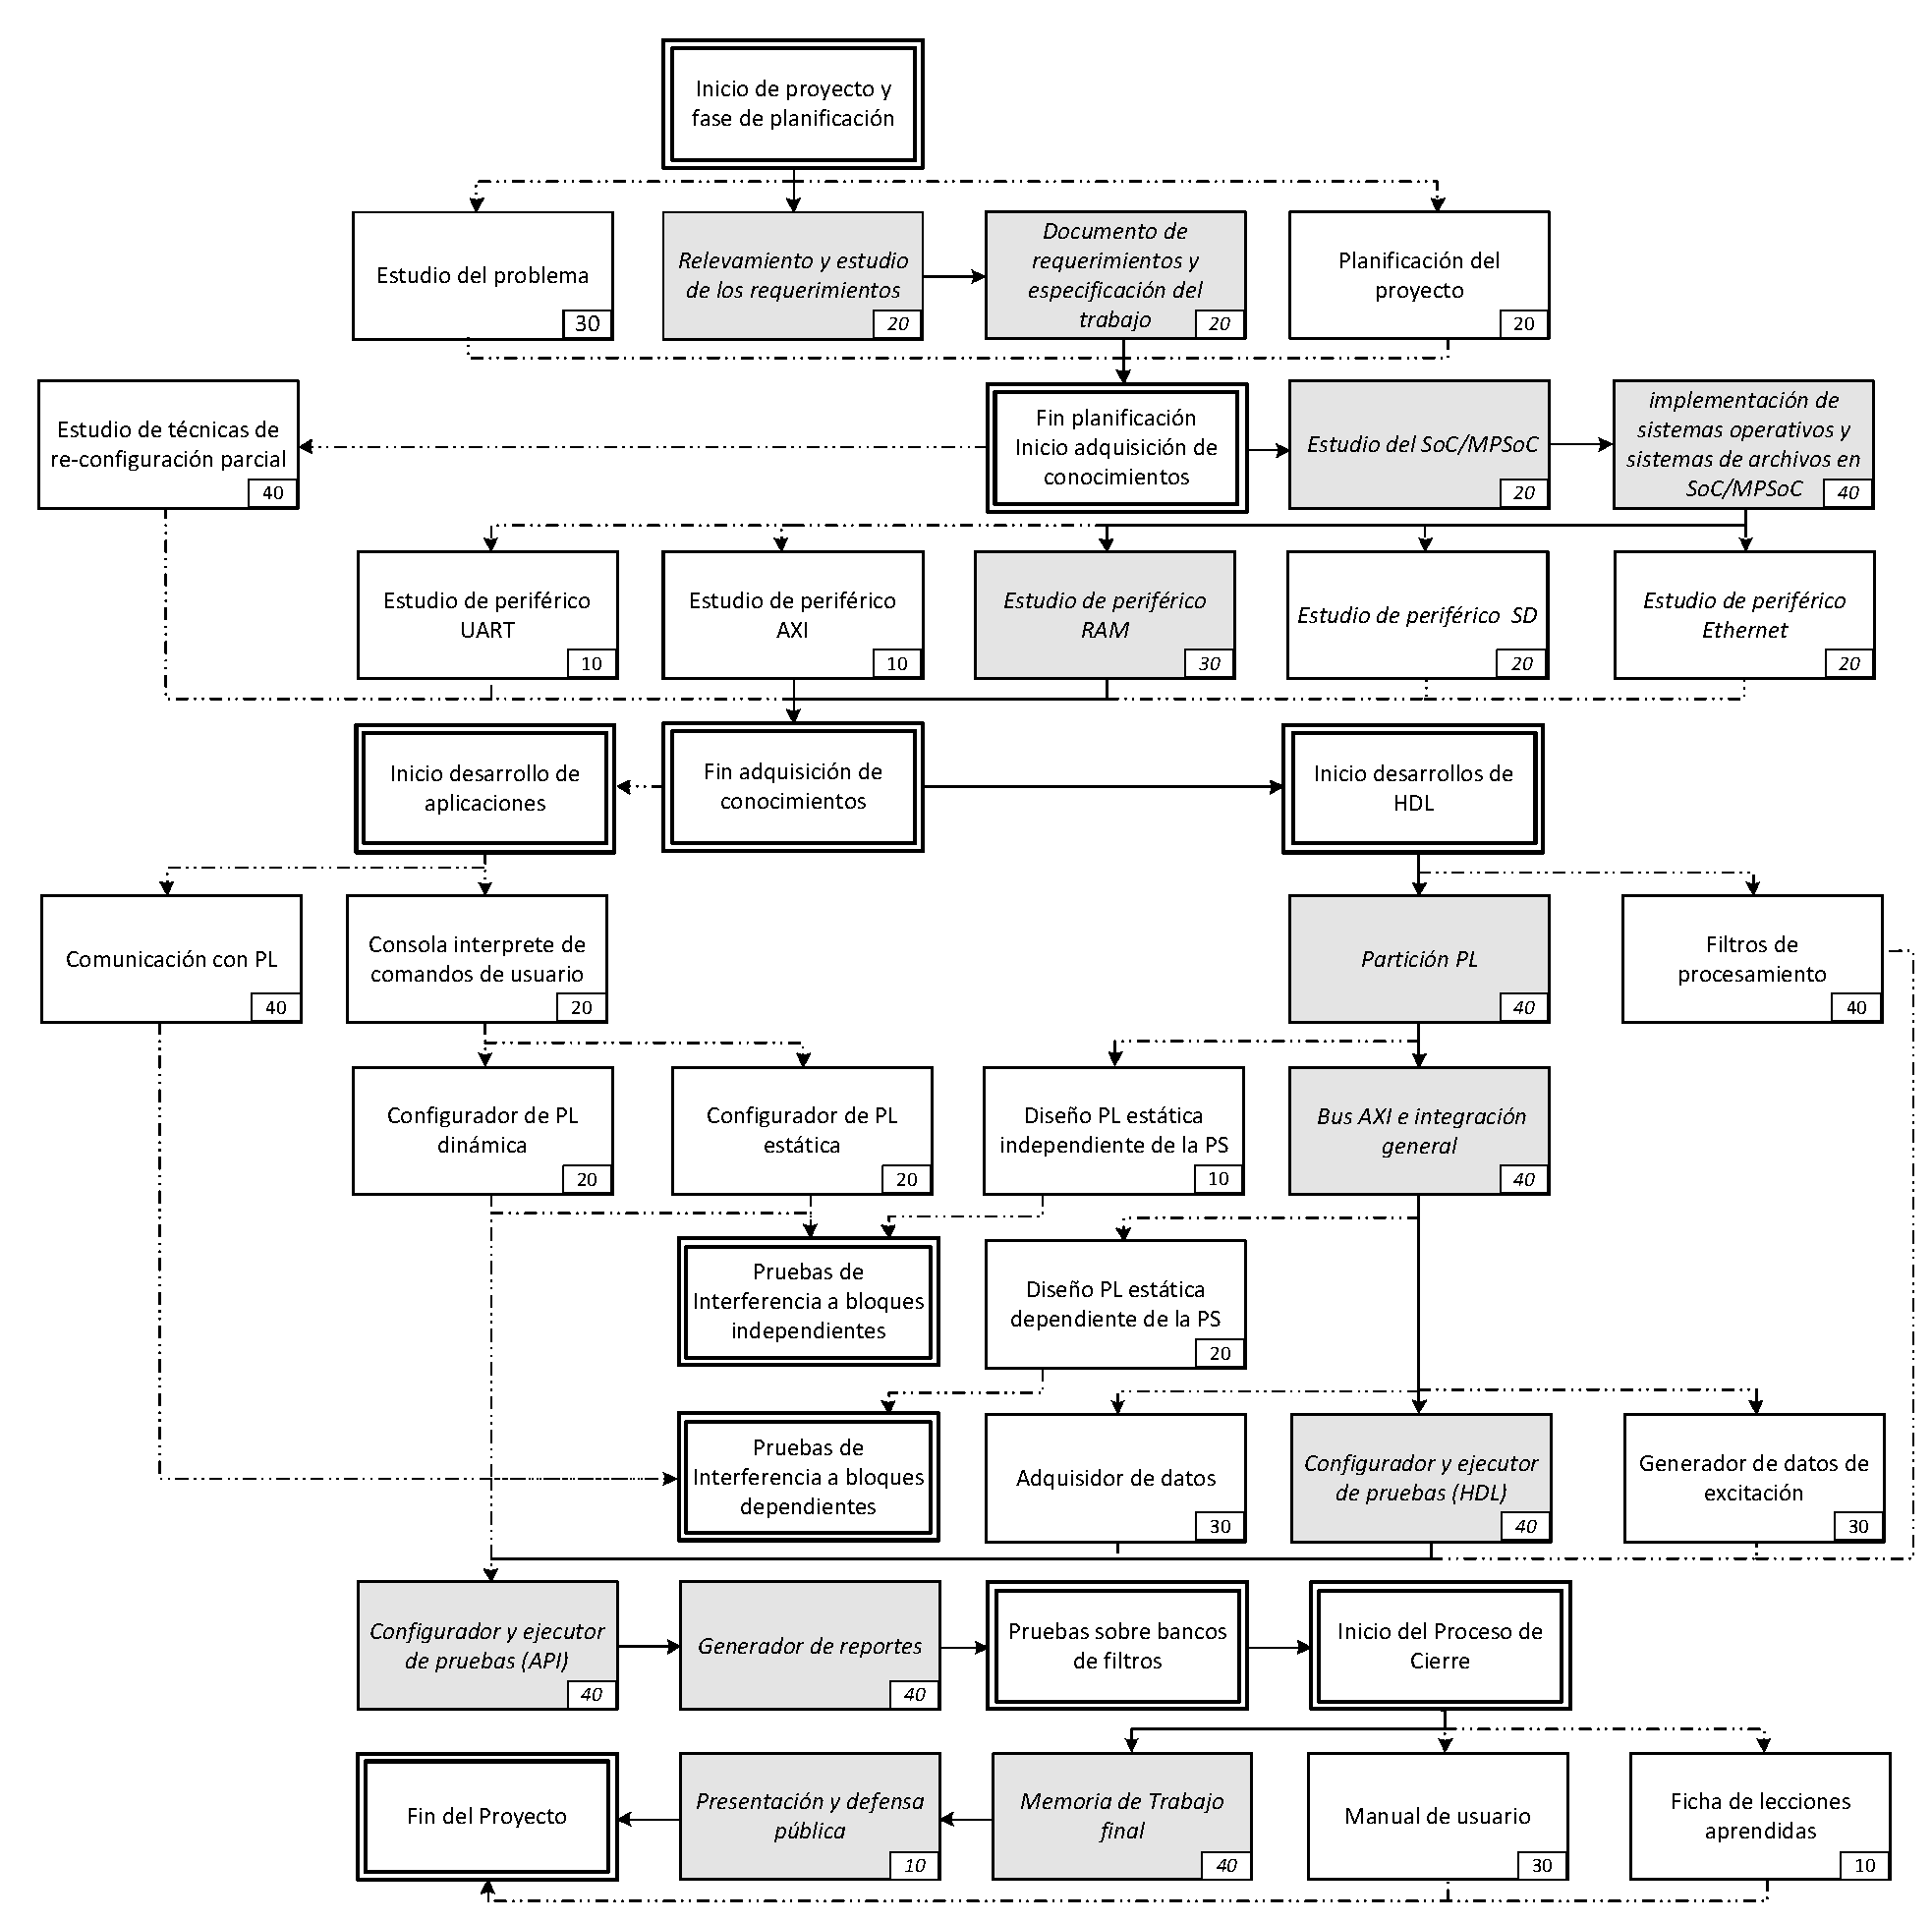
\includegraphics[width=1.05\textwidth]{./Figuras/AoN.pdf}
\caption{Diagrama en \textit{Activity on Node}.}
\label{fig:AoN}
\end{figure}

\clearpage

\section{11. Diagrama de Gantt}
\label{sec:gantt}

En la figura \ref{fig:diagGantt_faseinicial} y la figura \ref{fig:diagGantt_fasefinal} se muestra el diagrama de Gantt del proyecto, el mismo fue obtenido configurando la jornada laboral de 15 horas semanales.

En el diagrama de Gantt no se observan tareas realizadas de manera paralela,  esto se debe a que el proyecto cuenta con un único recurso. Por lo que, queda evidenciada una diferencia con el diagrama de AoN, en donde queda de manifiesto la dependencia entre las tareas según su relación técnica óptima.

\clearpage
%\begin{landscape}

\begin{figure}[h]
\centering 
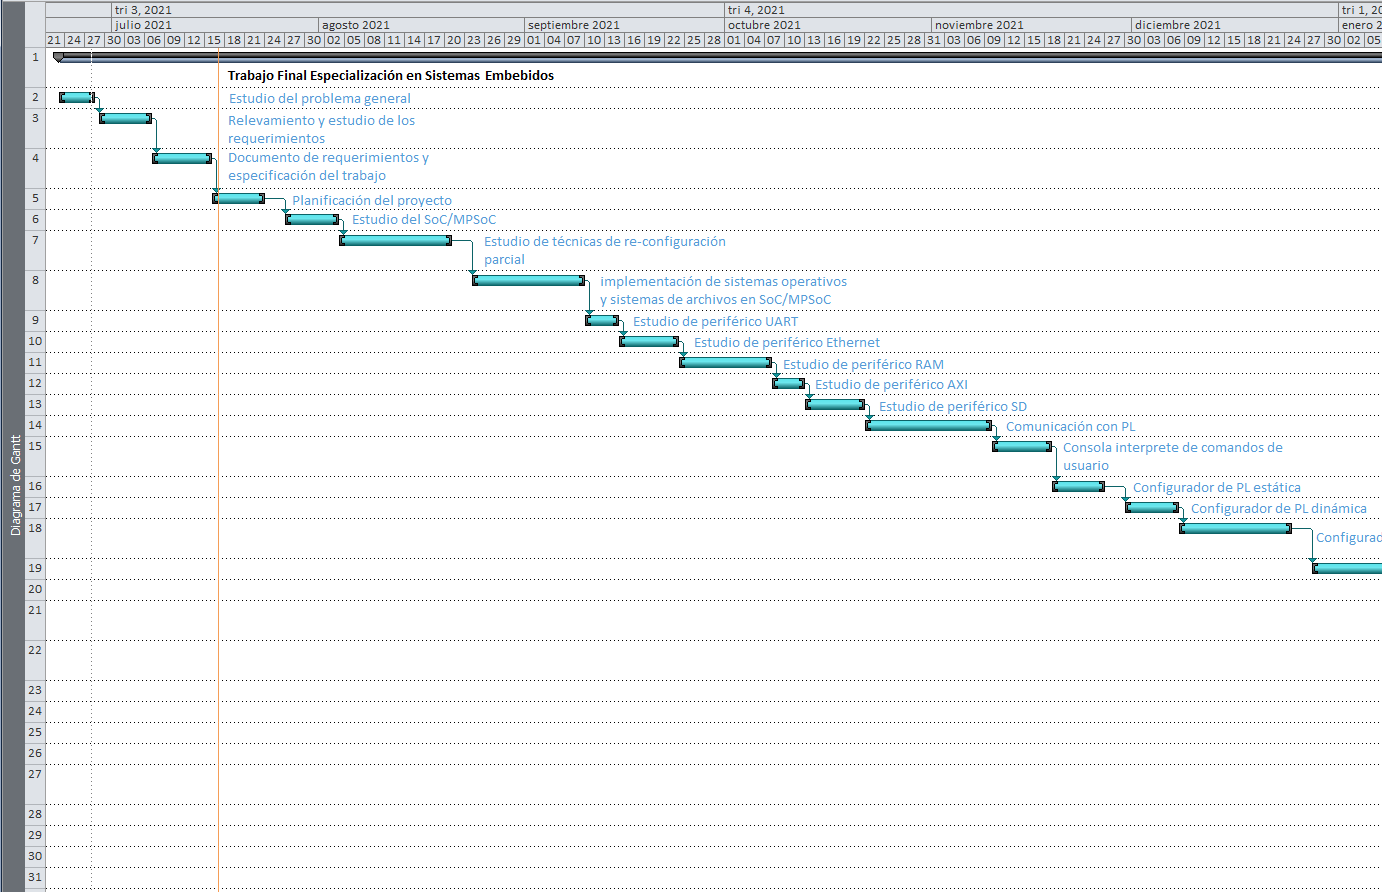
\includegraphics[angle=90, height=0.98\textheight]{./Figuras/Gantt-real_part1.png}
\caption{Diagrama de Gantt fase inicial.}
\label{fig:diagGantt_faseinicial}
\end{figure}

\begin{figure}[h]
\centering 
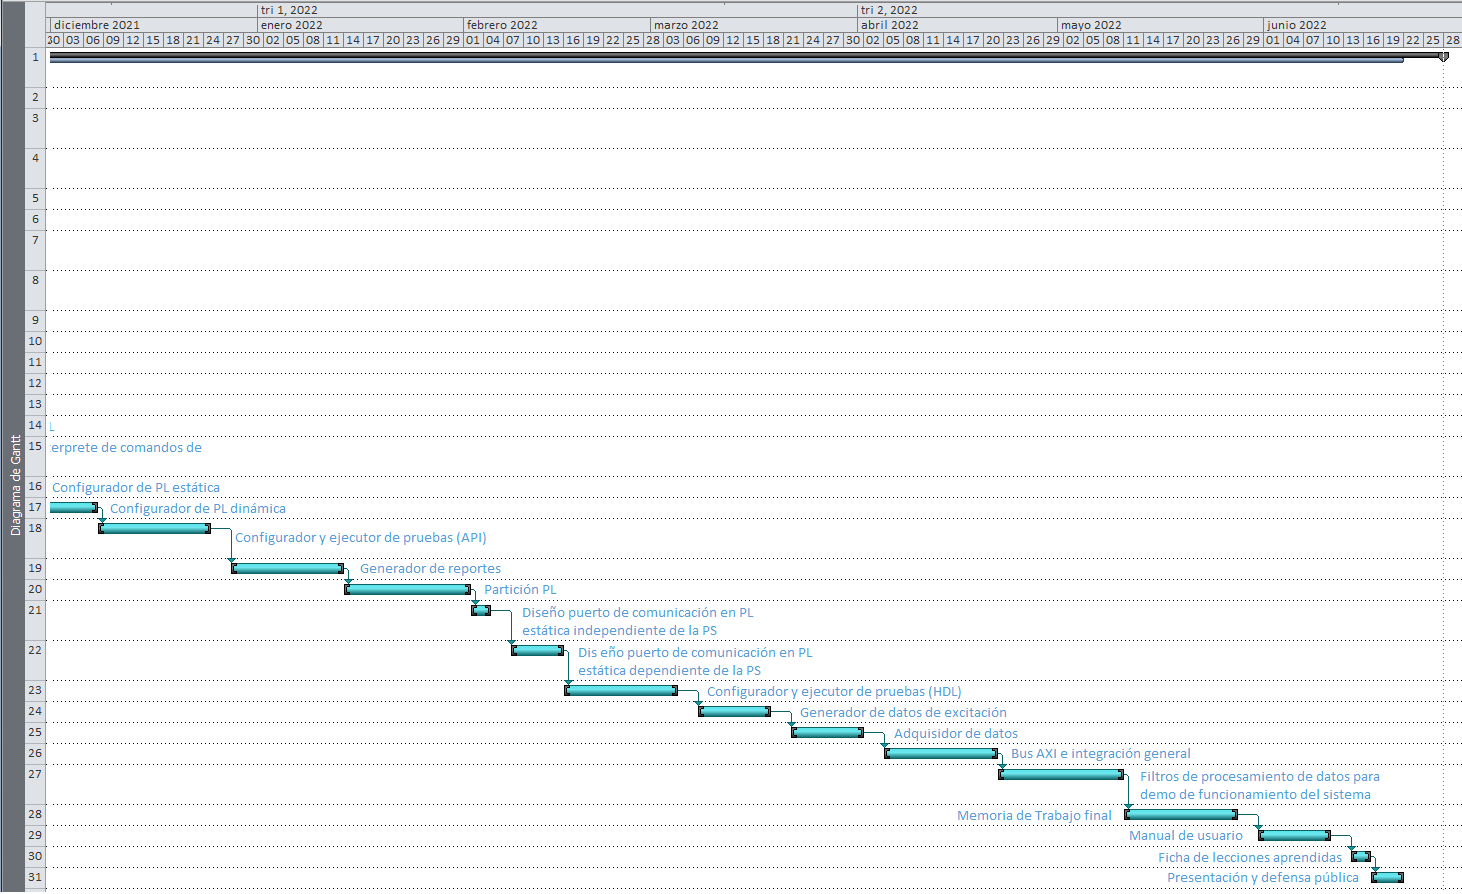
\includegraphics[angle=90, height=0.98\textheight]{./Figuras/Gantt-real_part2.png}
\caption{Diagrama de Gantt fase final.}
\label{fig:diagGantt_fasefinal}
\end{figure}

%\end{landscape}
\clearpage

\section{12. Presupuesto detallado del proyecto}
\label{sec:presupuesto}

\begin{table}[htpb]
\centering
\begin{tabularx}{\linewidth}{@{}|X|c|r|r|@{}}
\hline
\rowcolor[HTML]{\tablecolor} 
\multicolumn{4}{|l|}{\cellcolor[HTML]{\tablecolor}COSTOS DIRECTOS} \\ \hline
\rowcolor[HTML]{\tablecolor} 
Descripción &
  \multicolumn{1}{c|}{\cellcolor[HTML]{\tablecolor}Cantidad} &
  \multicolumn{1}{c|}{\cellcolor[HTML]{\tablecolor}Valor unitario [\$]} &
  \multicolumn{1}{c|}{\cellcolor[HTML]{\tablecolor}Valor total [\$]} \\ \hline
Ingeniería & 
  \multicolumn{1}{c|}{800 horas} &
  \multicolumn{1}{c|}{3.000} &
  \multicolumn{1}{c|}{2.400.000} \\ \hline
Imprevistos &
  \multicolumn{1}{c|}{} &
  \multicolumn{1}{c|}{} &
  \multicolumn{1}{c|}{160.000} \\ \hline
\multicolumn{3}{|l|}{SUBTOTAL} &
  \multicolumn{1}{c|}{2.560.000} \\ \hline
\rowcolor[HTML]{\tablecolor} 
\multicolumn{4}{|l|}{\cellcolor[HTML]{\tablecolor}COSTOS INDIRECTOS} \\ \hline
\rowcolor[HTML]{\tablecolor} 
Descripción &
  \multicolumn{1}{c|}{\cellcolor[HTML]{\tablecolor}Cantidad} &
  \multicolumn{1}{c|}{\cellcolor[HTML]{\tablecolor}Valor unitario [\$]} &
  \multicolumn{1}{c|}{\cellcolor[HTML]{\tablecolor}Valor total [\$]} \\ \hline
Costos indirectos &  &  &
   \multicolumn{1}{c|}{1.320.000} \\ \hline
\multicolumn{3}{|l|}{SUBTOTAL} &
  \multicolumn{1}{c|}{1.320.000} \\ \hline
  \rowcolor[HTML]{\tablecolor} 
  \multicolumn{4}{|l|}{\cellcolor[HTML]{\tablecolor}MATERIALES} \\ \hline
  \rowcolor[HTML]{\tablecolor} 
  Descripción &
	\multicolumn{1}{c|}{\cellcolor[HTML]{\tablecolor}Cantidad} &
	\multicolumn{1}{c|}{\cellcolor[HTML]{\tablecolor}Valor unitario [\$]} &
	\multicolumn{1}{c|}{\cellcolor[HTML]{\tablecolor}Valor total [\$]} \\ \hline
ZCU102 Development Board / ZedBoard & 
	\multicolumn{1}{c|}{1} &
	\multicolumn{1}{c|}{249.000} &
	\multicolumn{1}{c|}{249.000} \\ \hline
PC de desarrollo &
	\multicolumn{1}{c|}{1} &
	\multicolumn{1}{c|}{300.000} &
	\multicolumn{1}{c|}{300.000} \\ \hline
  \multicolumn{3}{|l|}{SUBTOTAL} &
	\multicolumn{1}{c|}{549.000} \\ \hline
\rowcolor[HTML]{\tablecolor}
\multicolumn{3}{|l|}{TOTAL} &
\multicolumn{1}{c|}{\projectcost}  \\ \hline
\end{tabularx}%
\caption{Presupuesto del proyecto.}
\end{table}

\clearpage

\section{13. Gestión de riesgos}
\label{sec:riesgos}

\begin{enumerate}[]
	\item Identificación de los riesgos y estimación de sus consecuencias:
	\begin{enumerate}[$\text{Riesgo}$ 1:, leftmargin=*,align=left] 
		
		\item Se cuenta con solo una ZedBoard propiedad del responsable del trabajo.
		\begin{itemize}
			\item Severidad (S): 9
			
			La pérdida, extravío o rotura de la placa de desarrollo generaría una imposibilidad de continuar con el avance del diseño en etapas avanzadas del proyecto.
			\item Probabilidad de ocurrencia (O): 4
			
			El hardware de desarrollo puede sufrir averías dado que es utilizado en un escritorio y no en un laboratorio. Así mismo, puede extraviarse o ser robado.
		\end{itemize}

		\item Recurso único de ejecución del proyecto.
		\begin{itemize}
			\item Severidad (S): 10
			
			Se cuenta con un solo recurso para realizar las tareas. El mismo trabaja 45 horas semanales. Por lo que, las 15 horas semanales para la ejecución del proyecto provienen de su tiempo libre y podrían surgir inconvenientes de índole personal.
			\item Probabilidad de ocurrencia (O): 2
			
			Se debe a que son hechos fortuitos, no conocidos previamente por lo que la probabilidad de ocurrencia es baja.
		\end{itemize}

		\item Licencias de entornos de desarrollo.
		\begin{itemize}
			\item Severidad (S): 7
			
			Entornos de desarrollo como Vivado y HDL Coder cuentan con licencias de pago para su utilización. No contar con las mismas podrían hacer que el tiempo de desarrollo suba.
			\item Probabilidad de ocurrencia (O): 4
			
			INVAP cuenta con las licencias en estos momentos, pero la renovación de las mismas son externas a este proyecto. 
		\end{itemize}

		\item Recurso sin experiencia en el manejo de sistemas operativos y aplicaciones en sistemas operativos.
		\begin{itemize}
			\item Severidad (S): 6
			
			El desarrollo necesita que se generen varias aplicaciones que se ejecutan dentro de un sistema operativo.
			\item Probabilidad de ocurrencia (O): 8
			
			El recurso ejecutor del proyecto tiene poca experiencia manejando sistemas operativos.
		\end{itemize}

		\item Dificultades funcionales entre PL estática y PL dinámica.
		\begin{itemize}
			\item Severidad (S): 7
			
			Se pueden encontrar limitaciones en la comunicación de ambas particiones de la lógica programable, esto podría generar un cambio en la arquitectura del banco de pruebas.
			\item Probabilidad de ocurrencia (O): 4
			
			Se leyeron publicaciones que indican que la forma de comunicar ambas particiones es correcta. Este hecho hace que la probabilidad de ocurrencia de esto sea baja. 
		\end{itemize}

		\item Tiempos de desarrollo.
		\begin{itemize}
			\item Severidad (S): 7
			
			Tiempos mal estimados en la planificación pueden influir directamente en la fecha de finalización del proyecto.
			\item Probabilidad de ocurrencia (O): 7
			
			En revisiones del plan de trabajo se hizo notar que probablemente el tiempo estimado para las tareas pueda ser muy optimista. 
		\end{itemize}

	\end{enumerate}

	\item Tabla de gestión de riesgos:

	\begin{table}[htpb]
	\centering
	\begin{tabularx}{\linewidth}{@{}|X|c|c|c|c|c|c|@{}}
	\hline
	\rowcolor[HTML]{\tablecolor} 
	Riesgo & S & O & RPN & S* & O* & RPN* \\ \hline
	Una sola ZedBoard propiedad del responsable del trabajo & 9 & 4  & \color{black}{\textbf{36}} & 9 & 1 & \color{black}{\emph{9}} \\ \hline
	Recurso único de ejecución del proyecto & 10 & 2 & \color{black}{20} & 10 & 2 & \color{black}{\emph{20}} \\ \hline
	Licencias de entornos de desarrollo & 7 & 4 & \color{black}{\textbf{28}} & 5 & 4 & \color{black}{\emph{20}} \\ \hline
	Recurso sin experiencia en el manejo de SO & 6 & 8 & \color{black}{\textbf{40}} & 6 & 2 & \color{black}{\emph{12}} \\ \hline
	Dificultades funcionales entre PL estática y PL dinámica & 7 & 4 & \color{black}{\textbf{28}} & 4 & 4 & \color{black}{\emph{16}} \\ \hline
	Tiempos de desarrollo & 7 & 7 & \color{black}{\textbf{49}} & 5 & 4 & \color{black}{\emph{20}} \\ \hline
	\end{tabularx}%
	\end{table}
	
	Se tomarán medidas de mitigación en los riesgos cuyos números de RPN sean mayores a RPN = 25. Nota: los valores marcados con (*) en la tabla corresponden luego de haber aplicado la mitigación.

	\item Plan de mitigación de los riesgos que originalmente excedían el RPN máximo establecido:
	
	\begin{enumerate}[$\text{Riesgo}$ 1:, leftmargin=*,align=left] 
		
		\item Se cuenta con solo una ZedBoard propiedad del responsable del trabajo.
		\begin{itemize}
			\item Severidad (S): 9
			
			No se registran cambios.
			\item Probabilidad de ocurrencia (O): 1
			
			\emph{Mitigación:} INVAP cuenta con numerosas placas de desarrollo que podrían ser utilizadas para el proyecto.
		\end{itemize}

		\item Recurso único de ejecución del proyecto.
		\begin{itemize}
			\item Severidad (S): 10
			
			No se registran cambios.
			\item Probabilidad de ocurrencia (O): 2
			
			No se registran cambios.
		\end{itemize}

		\item Licencias de entornos de desarrollo.
		\begin{itemize}
			\item Severidad (S): 5
			
			\emph{Mitigación:} se puede limitar el banco de filtros inicial a implementaciones simples que se encuentran en las librerías de IP Cores que no necesitan licencia de Vivado o HDL Coder.
			\item Probabilidad de ocurrencia (O): 4
			
			No se registran cambios.
		\end{itemize}
	
		\item Recurso sin experiencia en el manejo de sistemas operativos y aplicaciones en sistemas operativos.
		\begin{itemize}
			\item Severidad (S): 6
			
			No se registran cambios.
			\item Probabilidad de ocurrencia (O): 2
			
			\emph{Mitigación:} durante el transcurso de la especialización existen tres asignaturas sobre sistemas operativos y hay una optativa sobre aplicaciones para sistemas operativos.
		\end{itemize}

		\item Dificultades funcionales entre PL estática y PL dinámica.
		\begin{itemize}
			\item Severidad (S): 4
			
			\emph{Mitigación:} se realiza de manera temprana esta tarea para estimar si hay necesidad de ajustar la arquitectura del banco de pruebas.
			\item Probabilidad de ocurrencia (O): 4
			
			No se registran cambios.
		\end{itemize}

		\item Tiempos de desarrollo.
		\begin{itemize}
			\item Severidad (S): 4
			
			\emph{Mitigación:} se pueden disminuir las funcionalidades del primer prototipo del banco de pruebas y se tiene una flotabilidad en la ejecución del desarrollo. 
			\item Probabilidad de ocurrencia (O): 5
			
			\emph{Mitigación:} se puede hacer una evaluación temprana de los tiempos de desarrollo de acuerdo a lo que hayan llevado las tareas iniciales.
		\end{itemize}

	\end{enumerate}

\end{enumerate}

\clearpage

\section{14. Gestión de la calidad}
\label{sec:calidad}

\begin{enumerate}	
	\item Requerimientos de interfaces externas
		\begin{itemize}
			\item \emph{Verificación:} durante el desarrollo se realizan pruebas unitarias y de integración sobre cada una de las interfaces requeridas.
			\item \emph{Validación:} el cliente utilizará las interfaces externas para el uso del prototipo. 
		\end{itemize}
	
	\item Requerimientos de interfaces internas	
		\begin{itemize}
			\item \emph{Verificación:} restricciones de diseño que serán utilizadas para el desarrollo.
			\item \emph{Validación:} no son requerimientos funcionales por lo que el cliente no necesariamente debe validarlos. 
		\end{itemize}
	
	\item Requerimientos de almacenamiento de información (sistema de archivos)
	\begin{itemize}
		\item \emph{Verificación:} durante el desarrollo se realizan pruebas unitarias y de integración sobre cada una de las funcionalidades requeridas.
		\item \emph{Validación:} el cliente desarrolla pruebas sobre las funcionalidades sobre el producto final. 
	\end{itemize}
	
	\item Requerimientos generales de HDL
	\begin{itemize}
		\item \emph{Verificación:} estas restricciones de diseño serán tenidas en cuenta durante la realización de los bloques funcionales de HDL.
		\item \emph{Validación:} el cliente puede inspeccionar el código y validar los requerimientos de implementación. 
	\end{itemize}
	
	\item Requerimientos de HDL estático
	\begin{itemize}		
		\item \emph{Verificación:} durante el desarrollo se realizan pruebas unitarias y  de integración sobre cada bloques de HDL requeridos.
		\item \emph{Validación:} el cliente desarrolla pruebas sobre las funcionalidades sobre el producto final. 
	\end{itemize}
	
	\item Requerimientos de configuración del entorno de pruebas
	\begin{itemize}
		\item \emph{Verificación:} durante el desarrollo se realizan pruebas unitarias y de integración sobre cada una de las funcionalidades requeridas.
		\item \emph{Validación:} el cliente desarrolla pruebas sobre las funcionalidades sobre el producto final.
	\end{itemize}
		
	\item Requerimientos funcionales (ejecución de pruebas)
	\begin{itemize}
		\item \emph{Verificación:} durante el desarrollo se realizan pruebas unitarias y de integración sobre cada una de las funcionalidades requeridas.
		\item \emph{Validación:} el cliente desarrolla pruebas sobre las funcionalidades sobre el producto final.
	\end{itemize}

	\item Requerimientos de rendimiento
	\begin{itemize}
		\item \emph{Verificación:} se generan reportes en donde se muestra el tiempo de procesamiento.
		\item \emph{Validación:} se generan reportes en donde se muestra el tiempo de procesamiento.
	\end{itemize}

	\item Requerimientos de diseño
	\begin{itemize}
		\item \emph{Verificación:} por inspección visual se constata la utilización de la ZedBoard (o la placa dispuesta por el cliente). 
		\item \emph{Validación:} por inspección visual se constata la utilización de la ZedBoard (o la placa dispuesta por el cliente). 
	\end{itemize}

	\item Requerimientos de confiabilidad 
	\begin{itemize}
		\item \emph{Verificación:} durante el desarrollo se harán pruebas parciales. 
		\item \emph{Validación:} el cliente puede realizar un uso continuo del banco de pruebas para validar el requerimiento de confiabilidad.
	\end{itemize}

	\item Requerimientos de documentación
	\begin{itemize}
		\item \emph{Verificación:} durante el transcurso del desarrollo se generará información técnica parcial que será utilizada para confeccionar documentación requerida: Memoria Técnica, Ficha de lecciones aprendidas y Manual de usuario. 
		\item \emph{Validación:} el cliente realizará la lectura y revisión de los documentos a entregar: Plan de Trabajo, Memoria Técnica, Ficha de lecciones aprendidas y Manual de usuario.
	\end{itemize}
\end{enumerate}

\clearpage

\section{15. Procesos de cierre}    
\label{sec:cierre}

Los aspectos a trabajar durante todo el proceso de cierre son los siguientes:

\begin{itemize}
	\item Presentación oral de los principales resultados alcanzados.
	\item Contrastar el Plan de Trabajo con la Memoria Técnica, los documentos entregables e hitos parciales.
	\item Determinar el grado de cumplimiento de la planificación original. En lo referente a las estimaciones de esfuerzo previamente realizadas como los riesgos contemplados.
	\item Analizar el grado de cumplimiento de los requerimientos del proyecto.
	\item Identificar técnicas y procedimientos útiles e inútiles que se hayan implementado.
	\item Mostrar los problemas que surgieron y las soluciones encontradas para los mismos. 
	\item Se archivará toda la documentación de la gestión del proyecto para ser fácilmente reutilizada en la planificación de futuros proyectos.
	\item Establecer pautas para desarrollos futuros.
	\item Realizar los agradecimientos correspondientes.
\end{itemize}

La presentación de los tópicos previamente mencionados estará a cargo del \authortittle \authorname.

Al finalizar el proyecto se realiza una defensa publica donde estarán presentes:

\begin{itemize}
	\item El director del proyecto (\directortittle \supname).
	\item Los jurados.
	\item El equipo de trabajo del proyecto.
	\item El Responsable del proyecto (\authortittle \authorname).
\end{itemize}

La misma estará a cargo del Dr. Ing. Ariel Lutenberg en su calidad de Director de la Especialización en Sistemas Embebidos de la FIUBA.

\end{document}
